\subsection{Gradnja arhitekture}

Aplikacije ponavadi potrebujejo zunanje storitve za
pomoč pri delovanju.
Primeri storitev, ki jih zunanje aplikacije ponujajo so na primer
shramba, validacija podatkov, transformacija podatkov, pregled podatkov in podobno.
V naslednjih odsekih bomo pregledali zahteve aplikacije
in okoli nje zgradili arhitekturo iz zunanjih storitev, ki bodo zadoščale tem zahtevam.
Zgrajeno arhitekturo bomo prilagodili na izbrano okolje.

\subsubsection{Definicija zahtev aplikacije}

Big data aplikacije potrebutjo za svoje delovanje
tudi zunanje storitve, katere želimo postavljati skupaj z
aplikacijo.
V tem odseku bomo analizirali zahteve aplikacije in
iz njih zgradili arhitekturo.

Za začetek potrebujemo poslovno definicijo aplikacije.
Magistrska naloga predpostavlja, da je arhitektura
predstavljena v modelu ArchiMate, ampak od njega ni odvisna.
Arhitekturo bomo razvili za generično aplikacijo,
nato pa jo v poglavju~\ref{sec:uporaba-metodologije} uporabili
na primeru big data aplikacije.
Začnemo z definicijo big data aplikacije.
Aplikacija je sestavljena iz več procesov, kjer ima lahko
vsak proces več zahtev po zunanjih storitvah.
Generična predstavitev je predstavljena v sliki~\ref{fig:generic-arch-application}.

\begin{figure}[H]
    \centering
    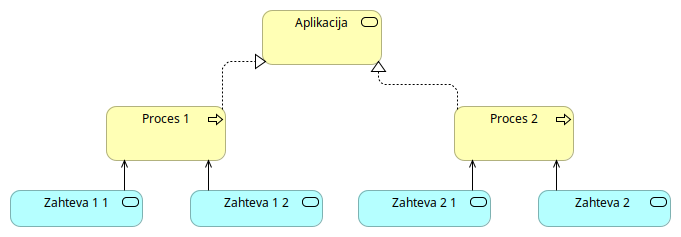
\includegraphics[width=0.9\textwidth]{img/gradnja/generic-arch-application.png}
    \caption{Predstavitev generične arhitekture v modelu Archimate.}
    \label{fig:generic-arch-application}
\end{figure}

Procesi in zahteve imajo lahko posebne lastnosti,
ki omejujejo izbor zunanjih storitev.
Lastnosti lahko definiramo sami, nekateri primeri so predstavljeni v tabeli 1 v članku~\cite{iterative_methodology},
kjer lastnosti storitev definirajo iz lastnosti big data,
ki smo jih predstavili v odseku~\ref{sec:big-data}.
Primeri lastnosti so na primer:
\begin{itemize}
    \item Volumen podatkov
    \item Hitrost podatkovnih tokov
    \item Raznolikost podatkov
    \item Zaupanje v podatke
    \item Strukturiranost podatkov
\end{itemize}

Lastnosti so lahko prisotne ali ne, na primer ali neka baza podpira nestrukturirane podatke ali ne,
ter prisotne na spektru, na primer kako hitro deluje.
Za arhitekturo v tem poglavju želimo, da bo aplikacija visoko dostopna.
V naši generični predstavitvi ta primer predstavimo s procesom 1 in pomeni,
da mora biti proces 1 in njegove zahteve visoko dostopni.
Dodana omejitev je predstavljena v sliki~\ref{fig:generic-arch-application-labels}.

\begin{figure}[H]
    \centering
    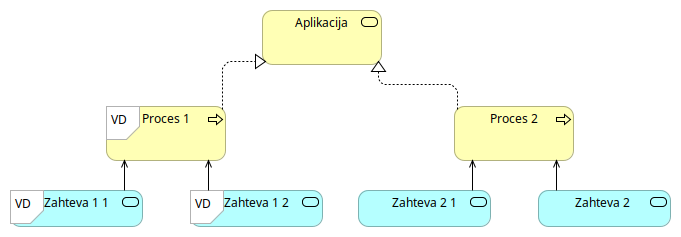
\includegraphics[width=0.9\textwidth]{img/gradnja/generic-arch-application-labels.png}
    \caption{Arhitektura z lastnostjo zahtev in procesov.}
    \label{fig:generic-arch-application-labels}
\end{figure}

V naslednjem koraku izpolnimo zahteve.
V prejšnjem koraku smo zahteve označili z lastnostmi in sedaj je naša
izbira tehnologij omejena na tiste, ki ustrezajo tem lastnostim.
Med ustreznimi tehnologijami se odločimo za tisto,
ki najbolj ustreza še drugim zahtevam, ki ne izvirajo nujno samo iz
same aplikacije, na primer da izberemo tehnologijo, ki jo naše podjetje
že pozna.
Po izbiri dodamo zunanje storitve v arhitekturo.
Ena storitev lahko zadostuje več zahtevam,
če zadostuje tudi njihovim lastnostim.
Arhitektura po dodatku storitev je predstavljena v sliki~\ref{fig:generic-services}.

\begin{figure}[H]
    \centering
    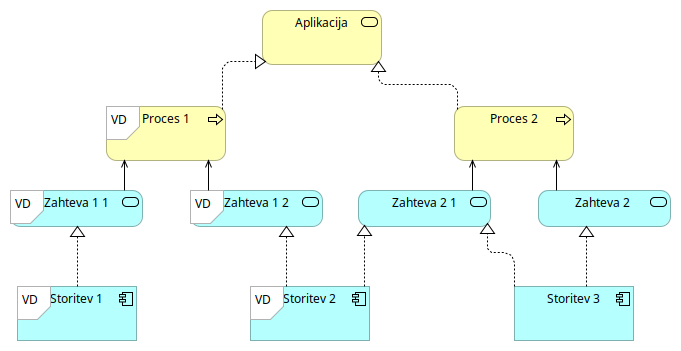
\includegraphics[width=0.9\textwidth]{img/gradnja/generic-services.png}
    \caption{Arhitektura s storitvami.}
    \label{fig:generic-services}
\end{figure}

V naslednjem odseku predstavimo primere tehnologij in njihove lastnosti.
Predstavili bomo par tehnologij iz vsake skupine in predstavili skupine na splošno.

\subsubsection{Izbira storitev}
V tem odseku predstavimo skupine orodij,
ki se pogosto uporabljajo pri delu z big data.
Skupine opišemo in predstavimo nekaj tehnologij,
ki spadajo v posamezno skupino.
Pri vsaki skupini napišemo lastnosti, katere tehnologije v njej zagotavljajo.

\paragraph{Obdelava podatkovnih tokov}
Zaradi povečanja količine in hitrosti podatkov potrebujemo nove tehnologije,
ki lahko podatke hitro obdelajo in pošljejo naprej.
Pri tem želimo, da so tehnologije visoko dostopne in da ponujajo zagotovila dostavljanja.
Delo s podatkovnimi tokovi ločimo na delo s
podatkovnimi paketi in delo s pravimi podatkovnimi tokovi.
Glavna razlika je, da podatkovne tokove uporabljamo,
ko imajo sveži podatki zelo veliko vrednost, ki hitro pada,
na primer opozorila o potresih.
Razlike so bolj podrobno predstavljene v tabeli~\ref{tab:stream-batch}.

\begin{table}[H]
    \centering
    \begin{tabularx}{\textwidth}{S L L}
                          & Podatkovni paketi          & Podatkovni tokovi                                                                  \\ \hline
        Podatki           & Podatkovni paketi.         & Tok svežih podatkov ali posodobitev.                                               \\
        Velikost podatkov & Znana v naprej in omejena. & Neskončna ali ni znana v naprej.                                                   \\
        Strojna oprema    & Več CPU.                   & Večinoma en CPU in omejena količina spomina.                                       \\
        Shramba           & Baza.                      & Ni shrambe, ali večina shranjena v spominu.                                        \\
        Procesiranje      & Več krogov procesiranja.   & En ali par krogov.                                                                 \\
        Trajanje          & Dolgo.                     & Par sekund ali milisekund.                                                         \\
        Aplikacije        & Pogosta uporaba.           & Izluščenje podatkov iz spleta, nadziranje prometa, obdelava podatkov iz senzorjev.
    \end{tabularx}

    \caption{Primerjava procesiranja podatkovnih tokov in podatkovnih paketov.
        Primerjava je povzeta po tabeli 1 iz~\cite{stream_analysis_systematic_literature_review}.}
    \label{tab:stream-batch}
\end{table}

Zagotovila dostavljanja ločimo na:
\begin{itemize}
    \item Največ enkrat, najlažja implementacija. Podatek se posreduje največ enkrat.
    \item Vsaj enkrat, srednje težka implementacija. Podatek se dostavi vsaj enkrat, kjer
          ob neuspeli dostavitvi ponovno poskušamo.
    \item Natanko enkrat, najtežja implementacija. Podatek se dostavi natanko enkrat.
\end{itemize}

Članek~\cite{stream_analysis_systematic_literature_review} v tabeli 9 predstavi
nekatere tehnologije za obdelavo podatkovnih tokov.
Povzetek tabele je v tabeli~\ref{tab:stream-tools}.

\begin{table}[H]
    \centering
    \begin{tabularx}{\textwidth}{L L L L L}
                        & Tip tokova                                & Zakasnitev & Propustnost & Zagotovitev dostavljanja \\ \hline
        BlockMon        & Tokovi                                    & Zelo nizka & Visoka      & Vsaj enkrat              \\
        Spark streaming & Paketi, tokovi in posamično               & Nizka      & Visoka      & Natanko enkrat           \\
        Apache Storm    & Tokovi                                    & Zelo nizka & Visoka      & Vsaj enkrat              \\
        Yahoo! S4       & Tokovi                                    & Nizka      & Nizka       & Natanko enkrat           \\
        Apache Samza    & Paketi in tokovi                          & Zelo nizka & Visoka      & Vsaj enkrat              \\
        Apache Flink    & Paketi, tokovi, posamično in interaktivno & Zelo nizka & Visoka      & Natanko enkrat           \\
        Apache Aurora   & Tokovi                                    & Nizka      & Visoka      & Vsaj enkrat
    \end{tabularx}

    \caption{Povzetek lastnosti orodij za procesiranje podatkovnih tokov.
        Tabela je povzeta po tabeli 9 iz~\cite{stream_analysis_systematic_literature_review}.}
    \label{tab:stream-tools}
\end{table}

Iz tabele~\ref{tab:stream-tools} lahko definiramo lastnosti zunanjih storitev,
glede na katere nato izberemo ustrezno orodje.
Vsaka napisana tehnologija ima še druge lastnosti, na primer na katere baze se lahko poveže.

\paragraph{Razpršen podatkovni sistem}

Pri delu z Big Data potrebujemo način za shranjevanje velikih količin podatkov.
En računalnik nima dovolj procesorske moči in predstalja eno točko odpovedi.
Želimo imeti način hrambe podatkov čez več računalnikov,
ki nam zagotavlja visoko dostopnost in odpornost na odpovedi.

Uporabimo lahko razpršene podatkovne sisteme~\cite{distributed_file_systems, big_data_review},
ki se trudijo biti tem bolj podobni navadnemu podatkovnemu sistemu,
samo da so uporabniki razpršenega podatkovnega sistema med sabo ločeni.
Tehnologija je namenjena dolgotrajni hrambi podatkov in njihovemu paralelnemu procesiranju.
Članek~\cite{analysiss_six_distributed} predstavi analizo šestih razpršenih podatkovnih sistemov.
Primerjava iz članka je predstavljena v tabeli~\ref{tab:distributed-fs-comparison}.

\begin{table}[H]
    \centering
    \begin{tabularx}{\textwidth}{L L L L}
                            & HDFS               & Ceph              & GlusterFS         \\ \hline
        Arhitektura         & Centralizirana     & Razpršena         & Decentralizirana  \\
        Dostopnost sistema  & Ena točka odpovedi & Visoka dostopnost & Visoka dostopnost \\
        Dostopnost podatkov & Visoka             & Visoka            & RAID              \\
        Replikacija         & Asinhrona          & Sinhrona          & Sinhrona          \\
        Delitev obremenitve & Avtomatsha         & Ročna             & Ročna
    \end{tabularx}

    \caption{Primerjava razpršenih podatkovnih sistemov.
        Primerjava je povzeta po tabeli 3.1 iz~\cite{analysiss_six_distributed}.}
    \label{tab:distributed-fs-comparison}
\end{table}

\paragraph{NoSQL}
Big Data je pogosto vsebuje nestrukturirane podatke,
katere želimo hitro shranjevati.
Za delo z njim se je razvila nova veja podatkovnih baz,
imenovanih NoSQL podatkovne baze.
Te baze ponujajo večjo hitrost, dostopnost in odpornost na
odpovedi, na račun konsistence podatkov~\cite{nosql,perf_comp_sql_nosql}.
NoSQL podatkovne baze delimo na več tipov,
kjer ima vsak tip svoje prednosti in slabosti~\cite{nosql_types,nosql_survey}.
Vsak tip NoSQL baz ima svoje prednosti in lastnosti, katere na kratko predstavimo v naslednjih odstavkih.

V ključ-vrednostnih podatkovnih bazah shranjujemo podatke na ključe.
Struktura podatkov ni pomembna.
Moderne ključ-vrednostne podatkovne baze dajejo prednost
skalabilnosti namesto konsistence podatkov.
Ta tip podatkovnih baz ne ponuja stikov kot SQL podatkovne baze,
saj lahko poizvedujemo samo po ključu.
V zameno za to omejitev nam ključ vrednostne podatkovne baze ponujajo hitre
poizvedbe in visoko skalabilnost~\cite{nosql_types}.

V dokumentinih podatkovnih bazah shranjujemo
podatke podobno kot v ključ-vrednostne podatkovne baze.
Podatke shranjujemo na določen ključ,
kjer so podatki v nekem standardnem formatu, npr. XML, PDF ali JSON.

V stolpičnih podatkovnih bazah je vsak ključ povezan z več stolpci,
ki so razpršeni med različnimi fizičnimi stroji.
Podatki so shranjeni tako, da omogočijo hitro agregacijo podatkov.

Grafovske podatkovne baze shranjujejo podatke v grafih,
kjer so informacije v obliki vozlišč in povezav.
Poudarek je na povezavah med podatki.
Te podatkovne baze je težje poganjati na gručah strojev in
večinoma imajo lastnosti ACID.
Uporabljajo se za podatke, ki tvorijo omrežja na primer
priporočilni sistemi, bioinformatika, socialna omrežja in podobno.

Članek~\cite{nosql} v tabeli 1 predstavi nekaj primerov NoSQL podatkovnih baz in jih med
sabo primerja.
Povzetek tabele je predstavljen v tabelah~\ref{tab:nosql-comparison-document}, \ref{tab:nosql-comparison-column}
in~\ref{tab:nosql-comparison-key-value}, posebaj pa predstavimo še grafovsko podatkovno bazo Neo4J.

\begin{table}[H]
    \centering
    \begin{tabularx}{\textwidth}{L S S}
        Lastnost                  & MongoDB & CouchDB \\ \hline
        MapReduce                 & Da      & Da      \\
        Atomarnost                & Pogojna & Da      \\
        Konsistenca               & Da      & Da      \\
        Izolacija                 & Ne      & Da      \\
        Transakcije               & Ne      & Ne      \\
        Horizontalna skalabilnost & Da      & Da      \\
    \end{tabularx}

    \caption{Primerjava dokumentinih NoSQL podatkovnih baz.
        Primerjava je povzeta po tabeli 1 iz članka~\cite{nosql}.}
    \label{tab:nosql-comparison-document}
\end{table}

\begin{table}[H]
    \centering
    \begin{tabularx}{\textwidth}{L S S S S }
        Lastnost                  & DynamoDB & HBase & Cassandra & Accumulo \\ \hline
        MapReduce                 & Da       & Da    & Da        & Da       \\
        Atomarnost                & Da       & Da    & Da        & Pogojna  \\
        Konsistenca               & Da       & Da    & Da        & Da       \\
        Izolacija                 & Da       & Ne    & Ne        & /        \\
        Transakcije               & Ne       & Da    & Ne        & Da       \\
        Horizontalna skalabilnost & Da       & Da    & Da        & Da       \\
    \end{tabularx}

    \caption{Primerjava stolpičnih NoSQL podatkovnih baz.
        Primerjava je povzeta po tabeli 1 iz članka~\cite{nosql}.}
    \label{tab:nosql-comparison-column}
\end{table}

\begin{table}[H]
    \centering
    \begin{tabularx}{\textwidth}{L S S}
        Lastnost                  & Redis & Riak \\ \hline
        MapReduce                 & Ne    & Da   \\
        Atomarnost                & Da    & Ne   \\
        Konsistenca               & Da    & Ne   \\
        Izolacija                 & Da    & Da   \\
        Transakcije               & Da    & Ne   \\
        Horizontalna skalabilnost & /     & Da   \\
    \end{tabularx}

    \caption{Primerjava ključ-vrednostnih NoSQL podatkovnih baz.
        Primerjava je povzeta po tabeli 1 iz članka~\cite{nosql}.}
    \label{tab:nosql-comparison-key-value}
\end{table}

Neo4J ne podpira MapReduce, podpira atomarnost, ponuja konsistenco in izolacijo,
ponuja transakcije in ni horizontalno skalabilen.

\subsubsection{Transformacija lastnosti}

\subsection{Posodabljanje arhitekture}